%!TEX root = ../report.tex

\begin{document}
\chapter{Methodology}\label{chap_methodology}
This chapter explains different experiments conducted to compare the two state-of-the-art uncertainty methods considered for this research work. Also, the experimental results are presented and analyzed.
\subsection{Datasets}
\subsubsection{Steering angle dataset}
The Udacity steering angle dataset (available in \cite{udacity_dataset}) consists of driving scene images captured by a set of three cameras(left, center, right) mounted behind the windshield of an ego vehicle. Along with the captured images, the dataset also contains steering angle, torque and vehicle speed values logged at that particular instance. The experiments conducted in this research work only utilizes the images captured the center camera and their corresponding steering angles expressed in radians. The data set contains driving scene images captured during different weather and traffic conditions(dataset samples can be found in \ref{fig_steer_data_samples}). The data set consists of 33,808 images in total and for the experiments conducted in this research, a train-validation-test split ratio of 80:5:15 is used. The following table gives further details about the dataset.

\begin{table}[h]
	\begin{tabular}{|c|c|c|c|c|c|}
		\hline
		\multicolumn{1}{|l|}{\multirow{2}{*}{\textbf{\begin{tabular}[c]{@{}l@{}}Dataset folder\\ identifier \end{tabular}}}} & \multirow{2}{*}{\textbf{Conditions}}                                                                                     & \multicolumn{4}{c|}{\textbf{Count}}                                                                                                                       \\ \cline{3-6} 
		\multicolumn{1}{|l|}{}                                                                                                                           &                                                                                                                          & \multicolumn{1}{l|}{\textbf{Train}} & \multicolumn{1}{l|}{\textbf{Validation}} & \multicolumn{1}{l|}{\textbf{Test}} & \multicolumn{1}{l|}{\textbf{Total}} \\ \hline
		HMB\_1                                                                                                                                           & Divided highway and sunny conditions                                                                                     & 3521                                & 220                                      & 660                                & 4401                                \\ \hline
		HMB\_2                                                                                                                                           & Two lane road and sunny conditions                                                                                       & 12637                               & 790                                      & 2369                               & 15796                               \\ \hline
		HMB\_4                                                                                                                                           & Divided highway segment                                                                                                  & 1579                                & 99                                       & 296                                & 1974                                \\ \hline
		HMB\_5                                                                                                                                           & Guard rail and two lane road                                                                                             & 3388                                & 212                                      & 635                                & 4235                                \\ \hline
		HMB\_6                                                                                                                                           & \begin{tabular}[c]{@{}c@{}}Divided multi-lane highway with a fair traffic \\ and shadows prevalent all over\end{tabular} & 5922                                & 370                                      & 1110                               & 7402                                \\ \hline
	\end{tabular}
\caption{\label{steer-angle-dataset} Train-validation-test split of the Udacity steering angle dataset}
\end{table}

\begin{figure}[h]
	\centering
	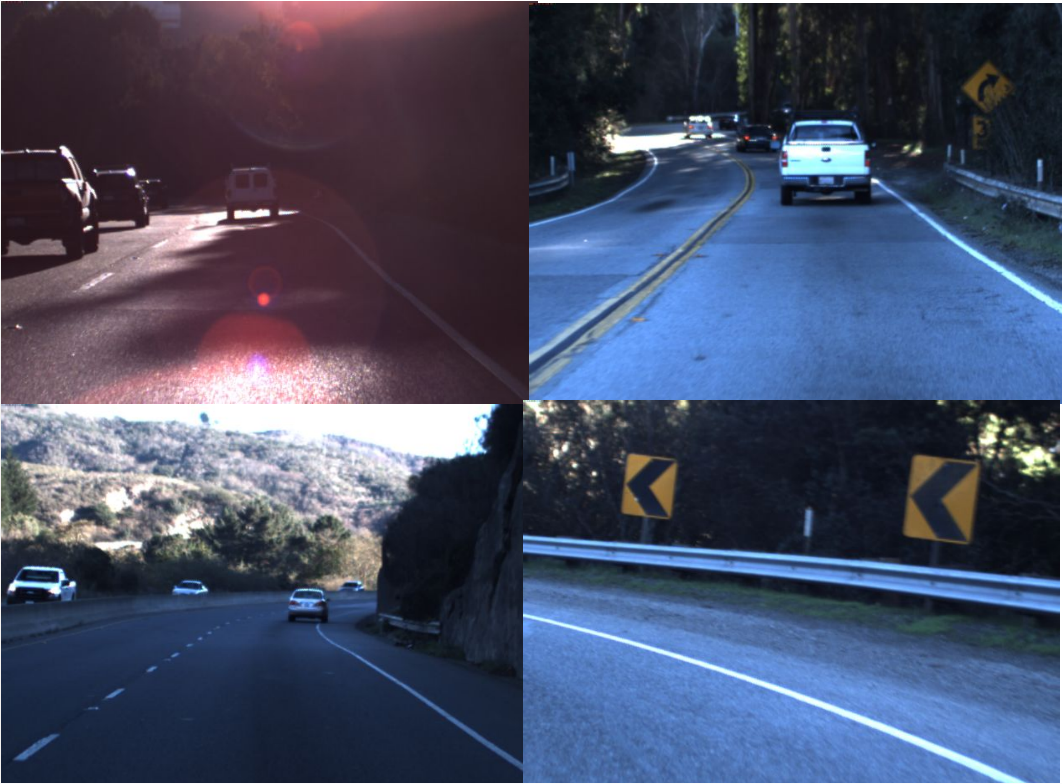
\includegraphics[scale=0.35]{steerdataset-samples}
	\caption{Sample images from the Udacity steering angle dataset. Image source: }
	\label{fig_steer_data_samples}
\end{figure}

Steering angle prediction is both a safety and time critical application which serves as an essential component of any autonomous vehicle. As enhancing functional safety in such applications is one of the key objectives of using uncertainty estimation methods, the steering angle data set is chosen for benchmarking the techniques considered for this research work.   
\subsection{Network architectures}
\subsubsection{Dronet}
Dronet, a residual convolutional network architecture is used for experiments conducted on the steering angle dataset. The Neural Network is primarily designed to safely navigate a drone by performing the tasks of steering angle prediction(regression) and collision detection(binary classification). However, for the experiments conducted in this research work the collision detection output is not required and therefore its corresponding output branch in the Neural Networks output layer is discarded. Figure \ref{fig_resnet8} depicts Dronet's architecture.

The model used for experiments takes a gray-scale input of size 200x200 and propagates it through a pair of convolution and max-pooling layers, three residual blocks, a dropout layer, a ReLU activation and finally a fully-connected(fc) layer which outputs predicted steering angles. When it comes to integrating MCDO\_ADF(described in \ref{general_framework}) with Dronet, new dropout layers are introduced before every convolutional layer at the test time. On the other hand, DER (described in \ref{der}) is integrated to Dronet by introducing three more output branches in the last fc layer for outputting parameters of the evidential distribution (described in \ref{sec_evidential_dist}).
\begin{figure}
	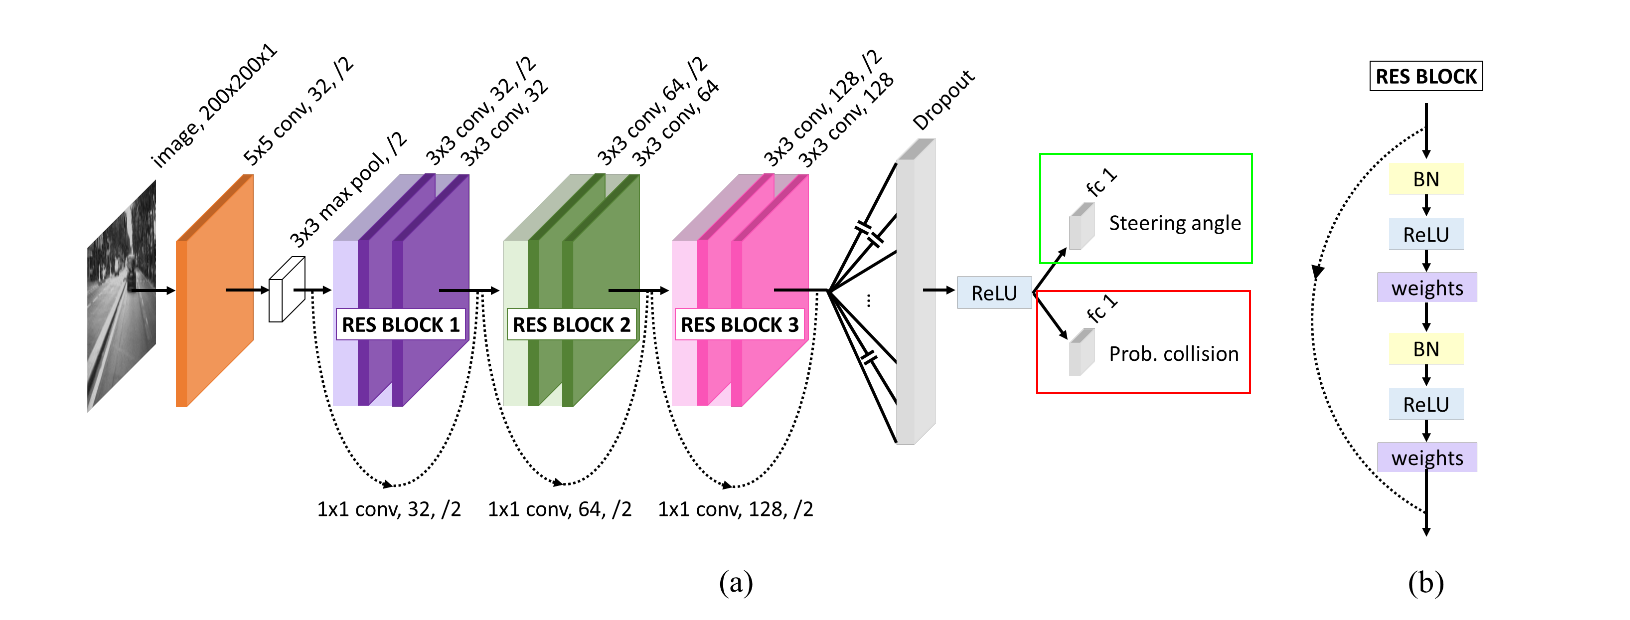
\includegraphics[scale=0.30]{resnet8}
	\caption{(a) Dronet architecture (b) Structure of every residual block . Collision classification output (bounded by the red box) is discarded and the steering angle prediction branch(bounded by the green box) is retained for this experiment.  Image source: }
	\label{fig_resnet8}
\end{figure}
 
\subsection{Training details}
\subsubsection{Dronet with steering angle dataset}
In order to benchmark the considered uncertainty estimation methods(MCDO\_ADF and DER), a set of three Dronet models are used: 1. Vanilla version of Dronet 2. MCDO\_ADF version of dronet with dropout layers after convolution layers 3. Evidential version of Dronet which uses the evidential loss function. Training details for those variants are provided in upcoming sections.

Choice of certain hyperparameter values remains unchanged for training all the three models and are listed in the table below.

\begin{table}[h]
	\begin{tabular}{|l|l|}
		\hline
		\textbf{Hyperparameter} & \textbf{Value}                                                                                                                                                                                                                            \\ \hline
		Input image size (hxwxc)                 & 200 x 200 x 1                                                                                                                                                                                                                                              \\ \hline
		Batch size                               & 32                                                                                                                                                                                                                                                         \\ \hline
		Training epochs                          & 100                                                                                                                                                                                                                                                        \\ \hline
		Learning rate                            & 0.001                                                                                                                                                                                                                                                      \\ \hline
		Dropout rate                             & 0.2                                                                                                                                                                                                                                                        \\ \hline
		Weight decay                             & 0.0001                                                                                                                                                                                                                                                     \\ \hline
		Learning rate decay                      & 0.00001                                                                                                                                                                                                                                                    \\ \hline
		Choice of optimizer                      & Adam                                                                                                                                                                                                                                                       \\ \hline
		Initializers                             & \begin{tabular}[c]{@{}l@{}}Kaiming-normal for Conv2D in residual blocks,   \\ Xavier-uniform for Conv2D, linear layers in non-residual blocks, \\ Constant initialization for batch normalization layers\\ (weights with 1 and biases with 0)\end{tabular} \\ \hline
	\end{tabular}
\end{table}


\subsubsection{Vanilla Dronet}
A simple dronet model predicts steering angle for the given image input. Training the model involves reduction of the Mean Squared Error (MSE) loss, which is popular choice for regression problems. Optimizing the MSE loss function intuitively means reduction of mean over euclidean distance (L2-Norm) between ground truth labels and predictions of observed data. The MSE loss function can be expressed as follows:

\begin{equation}
	\mathbf{L}(y,\hat{y})=\frac{1}{N}\sum_{i=0}^{N}(y-\hat{y}_i)^2
\end{equation} 
\begin{figure}[h]
	\centering
	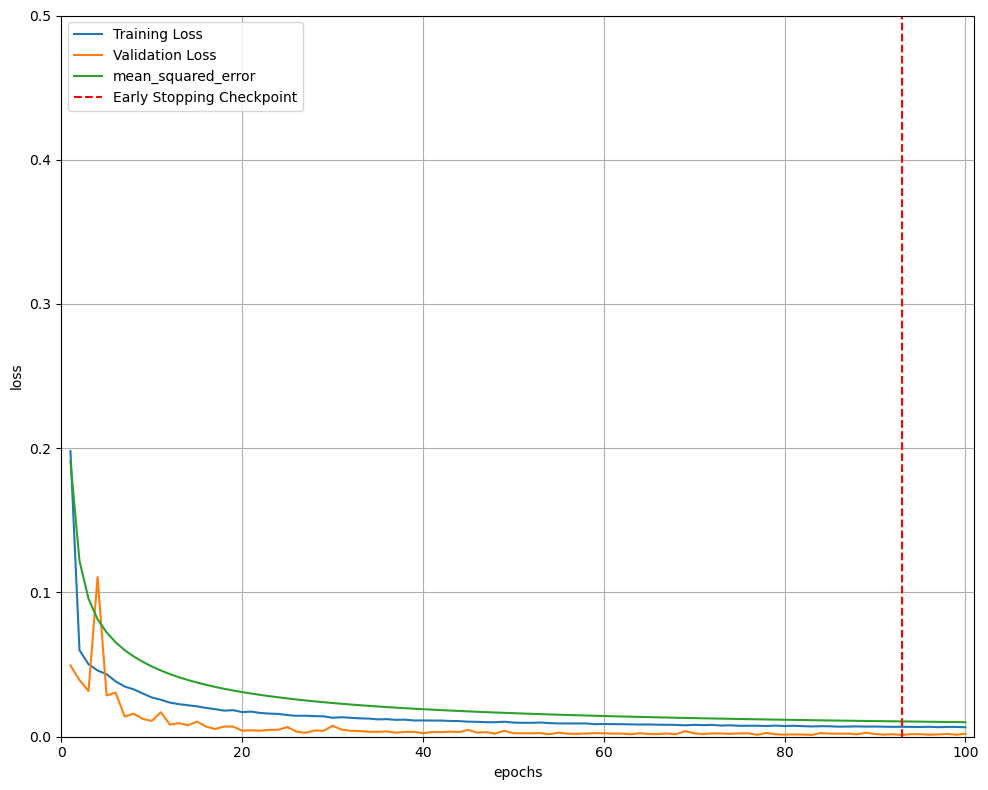
\includegraphics[scale=0.4]{dronet_mse_loss}
	\caption{Plot depicting the trend of Mean-Squared-Error loss while training vanilla Dronet}
	\label{fig_mse_loss_dronet}
\end{figure}

The technique of early stopping is used to avoid over-fitting, by saving model weights at the epoch corresponding to the least validation loss.

\subsubsection{MCDO\_ADF Dronet}
This variant of Dronet is trained to facilitate estimation of uncertainty associated with its predictions using the MCDO\_ADF technique. The training procedure for this variant remains unchanged from the Vanilla variant except for the  introduction of dropout after every convolution layer. Though it is sufficient to have the vanilla variant for applying this method, dropout was used during training with an intent to regularize the process.
\begin{figure}[h]
	\centering
	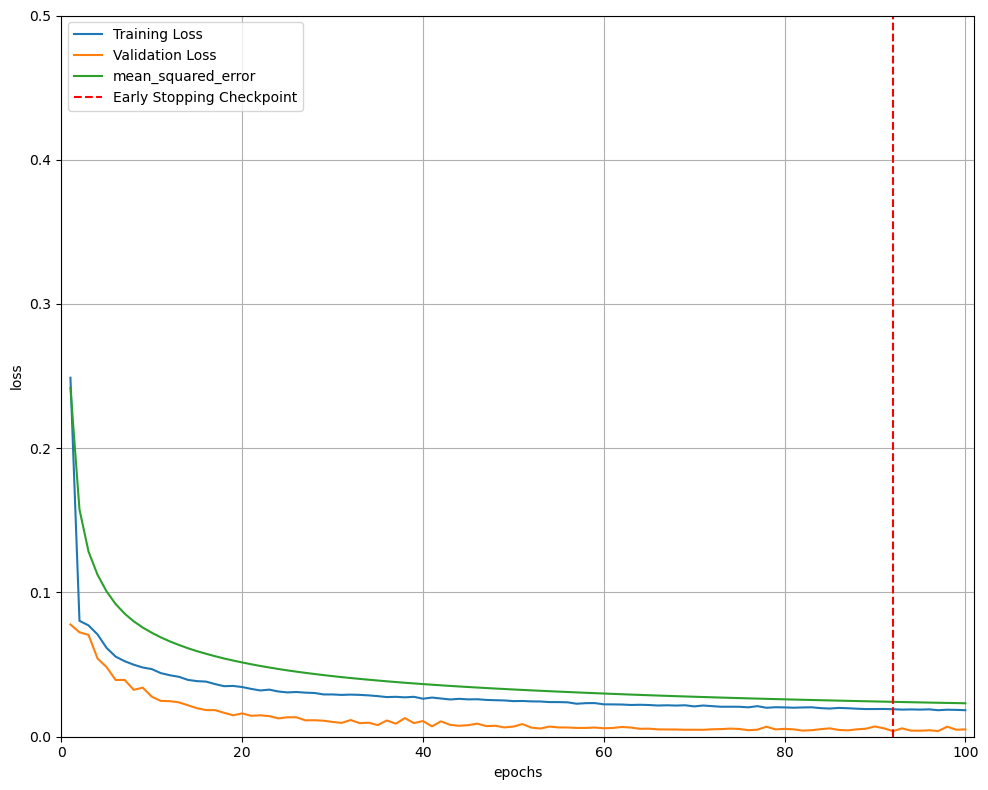
\includegraphics[scale=0.4]{dronet_MCDO_mse_loss_plot}
	\caption{Plot depicting the trend of Mean-Squared-Error loss while training MCDO\_ADF Dronet}
	\label{fig_mse_loss_mcdo_dronet}
\end{figure}

The inference procedure for MCDO\_ADF applied models is clearly explained in \ref{sec_mcdo_adf}. There are three hyper-parameters additionally required for the procedure: 1. Monte-Carlo(MC) sample count 2. Noise-variance 3. Minimum-variance. The value of MC sample count has a direct impact on the inference time as it determines number of forward passes for a given input to determine model uncertainty. For this experiment, we set its value to be 20 to replicate results provided in \cite{loquercio2020a}. Both the values of noise-variance and minimum variance are chosen to be 0.001. Noise variance indicates the level of sensor noise and minimum-variance signifies the minimum value of noise-variance to be propagated through every layer.

\subsubsection{Evidential Dronet}
The evidential Dronet model outputs parameters of the evidential distribution(described in the section \ref{sec_evidential_dist}) for a given input image. The distribution parameters can be in turn used to calculate prediction and uncertainty associated with it. Except for the choice of evidential loss function(described in \ref{sec_evi_learning_objectives}) for this model , training criteria remains unchanged from the vanilla variant.
\begin{figure}[h!]
	\centering
	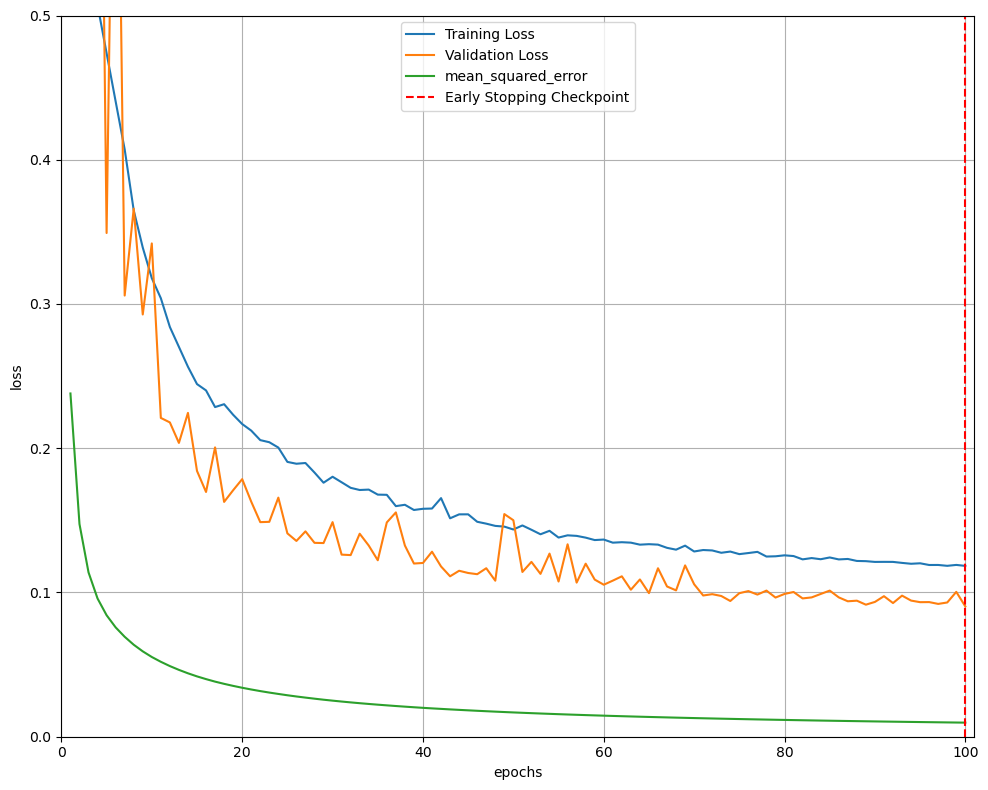
\includegraphics[scale=0.4]{dronet_evidential_loss_plot}
	\caption{Plot depicting the trend of evidential loss while training evidential Dronet}
	\label{fig_mse_loss_mcdo_dronet}
\end{figure}



